\chapter{Développement et résultats}

\section{Liste complète des solutions}

Comme indiqué et jutifié précédement, nous avons décidé d'utiliser l'outil \textbf{DialogFlow} de Google\cite{dialogflow} pour répondre à notre problématique principale, à savoir
le système de dialogue.\\

Nous avons décidé d'adopter une architecture client/serveur, classique mais efficace afin de gérer les traitements liés au \emph{DialogManager} uniquement coté serveur. Afin
de permettre à l'application client de communiquer avec notre agent assistant, nous avons choisis d'implémenter un Serveur REST écrit en \textbf{Node.js}\cite{node} en
utilisant le module \textbf{Express.js}\cite{express} qui permet de déployer rapidement un serveur REST scalable et de fournir une API simple et efficace.\\

Coté client, nous avons choisis de créer une application mobile en utilisant la technologie open-source \textbf{react-native}\cite{reactnative} de Facebook couplée
au framework \textbf{create-react-native-app}\cite{createnative} pour plusieurs raisons :
\begin{itemize}
    \item Permet de créer une application \emph{cross-plateform} (iOS et Android) ;
    \item Simple et rapide à déployer contrairement à une application native ;
    \item De la curiosité, tout simplement, étant donné que la problématique du sujet est indépendante de l'application client utilisée.
\end{itemize}

\section{Architecture}

En figure \ref{archi}, vous pouvez trouver un diagramme de déploiement qui récapitule le plus simplement et clairement possible l'ensemble de notre architecture.

\begin{figure}[H]
	\centering
		\centering
		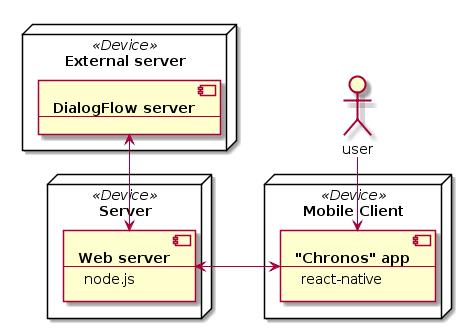
\includegraphics[width=0.9\textwidth]{../docs/conception/build/architectureDiagram.png}
        \caption{Architecture de notre solution}
        \label{archi}
\end{figure}


\section{Gestion de projet}

Pour la gestion du projet, nous avons choisi d'utiliser l'outil \textbf{Trello}\cite{trello} afin de décomposer le projet en différentes tâches et ainsi simplifier
la répartition du travail à effectuer ainsi que le développement.

\section{Développement}

\subsection{Côté Serveur}

\subsubsection{Système de dialogue}

Comme indiqué ci-dessus, nous utilisons \textbf{DialogFlow} pour gérer la logique du système de dialogue. DialogFlow propose en effet une interface web très simple à
l'intention du développeur qui lui permet de créer un \emph{chat bot} (i.e. agent conversationnel). Nous pouvons ainsi donner et configurer des \emph{intentions} à notre agent (figure \ref{intents}).\\

\begin{figure}[H]
    \centering
        \centering
        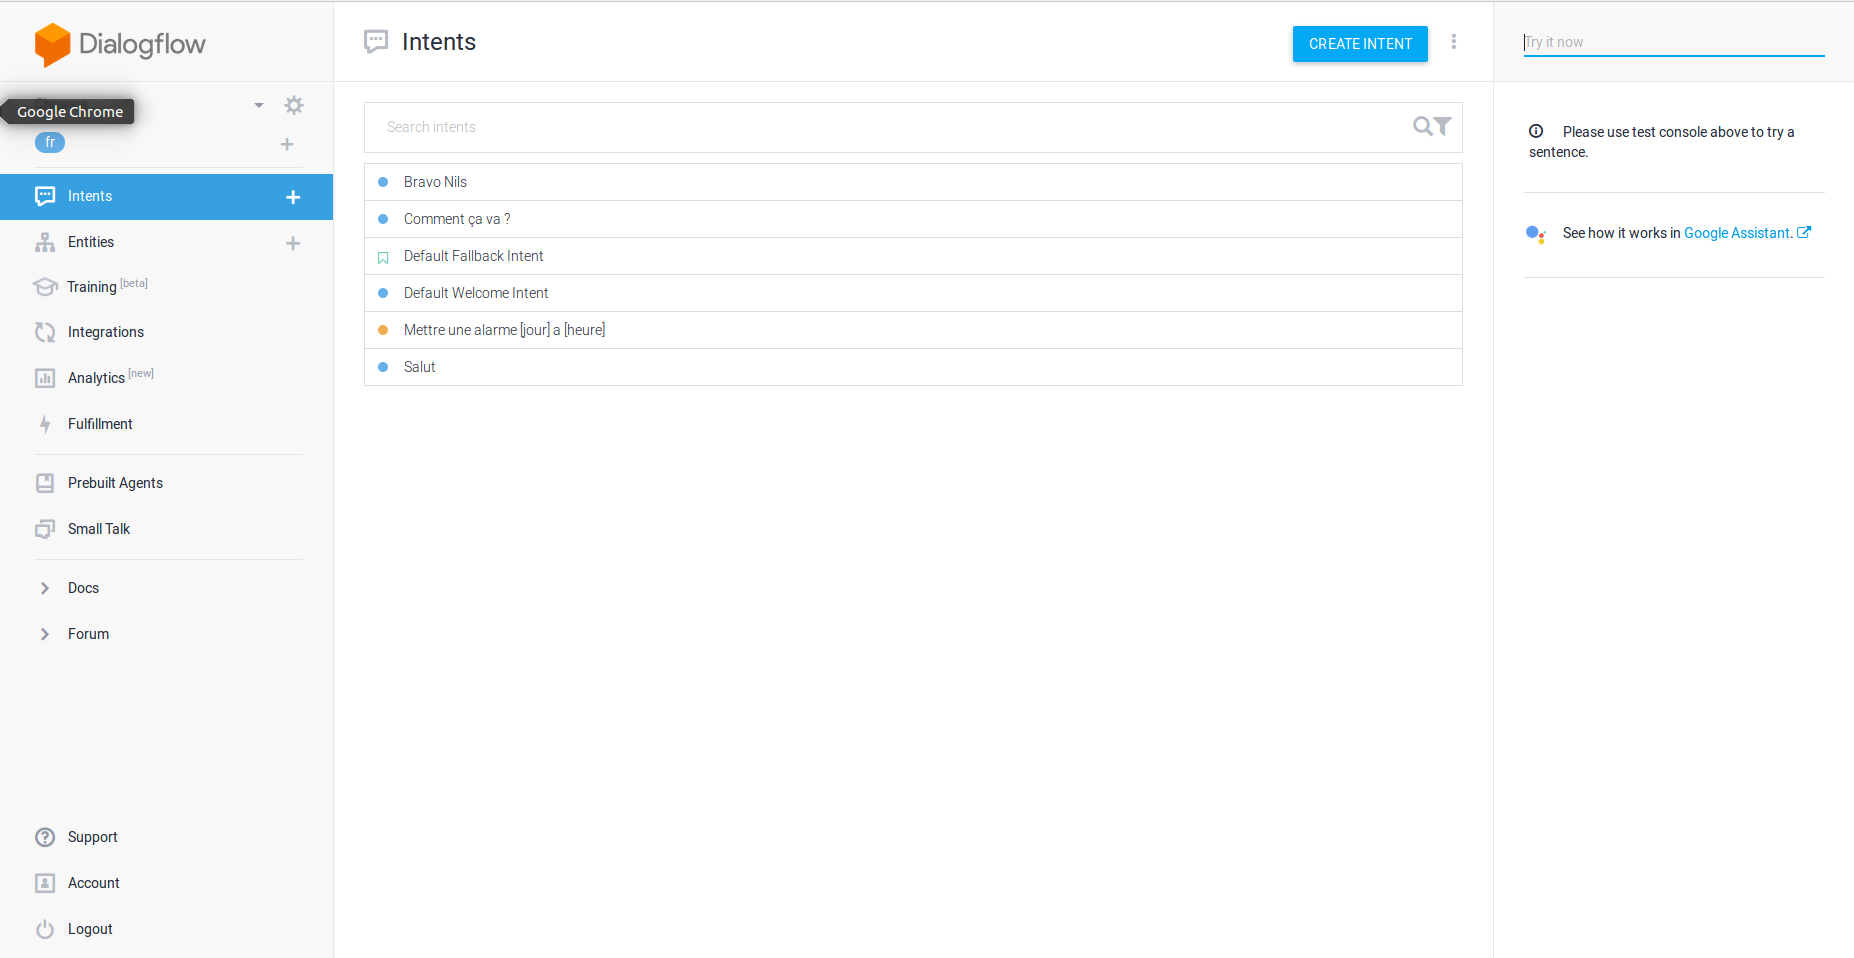
\includegraphics[width=1\textwidth]{images/dialogflow.png}
        \caption{Interface de DialogFlow}
        \label{intents}
\end{figure}

Notre principale intention (i.e. motivation) est de converser avec notre agent sur la programmation d'une alarme. Pour ceci, nous créons une \emph{Intent} (i.e. intention) dont
la configuration se fera en plusieurs étapes.\\

La première étape constitue une phase de \textbf{tagging} : nous allons écrire notre intention de programmer une alarme via plusieurs types de phrases possibles et différentes.
Dans chaque phrase nous allons indiquer à notre agent quels \textbf{tags} il doit systématiquement parser. Il devra parser 3 tags différents qui sont : [alarme], [date] et
[heure]. Un exemple est donné en figure \ref{tagging}.

\begin{figure}[H]
    \centering
        \centering
        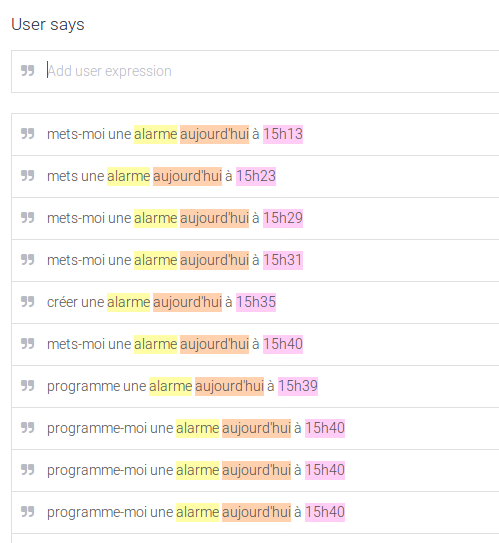
\includegraphics[width=0.7\textwidth]{images/intents.png}
        \caption{Phase de tagging}
        \label{tagging}
\end{figure}

Comme vous pouvez le constater à la figure \ref{action}, pour chacun des tags, nous indiquons s'il est obligatoire, son type et plusieurs réponses possibles de l'agent si jamais ce \emph{tag} est absent.\\

DialogFlow gère
très bien les notions de \textbf{contexte}, c'est pourquoi lorsqu'un dialogue débute avec notre agent, il va garder en mémoire les \emph{tags} qu'il aura extrait depuis le
début de la conversation. Il est donc très facile de réorienter l'utilisateur vers l'information manquante pour paramétrer une alarme.

\begin{figure}[H]
    \centering
        \centering
        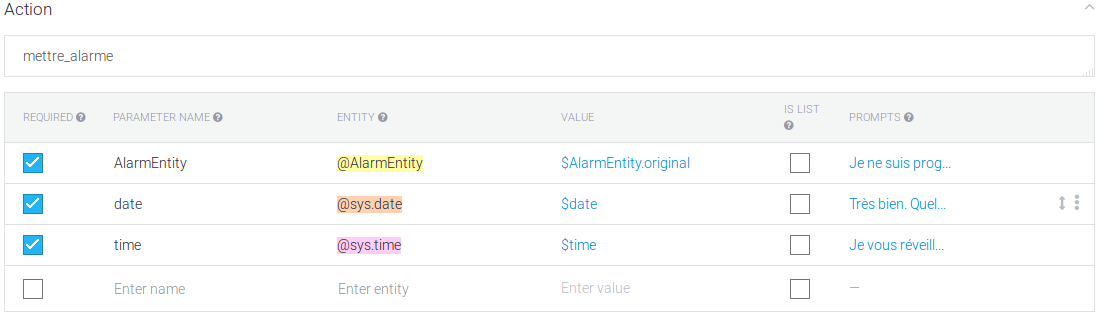
\includegraphics[width=\textwidth]{images/action.png}
        \caption{Les tags à extraire}
        \label{action}
\end{figure}

Finalement, nous devons configurer les différentes réponses possibles de l'agent lorsque tous les \emph{tags} d'une intention ont été reconnus. DialogFlow ayant gardé en mémoire
ces \emph{tags}, nous pouvons très facilement les ré-insérer dans la réponse de l'agent comme sur la figure \ref{answer}.

\begin{figure}[H]
    \centering
        \centering
        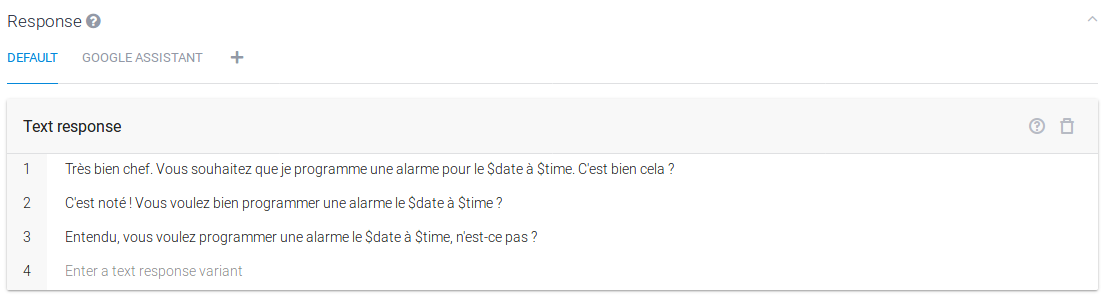
\includegraphics[width=1\textwidth]{images/answer.png}
        \caption{Réponses possibles de l'agent lorsqu'une intention est complète}
        \label{answer}
\end{figure}

Nous avons également configuré quelques autres \emph{intentions} basiques (demander à l'agent s'il va bien, lui dire bonjour, etc.) afin de rendre l'agent plus convivial
pour l'utilisateur.\\

DialogFlow possède également un onglet \og \emph{training} \fg{} (figure \ref{training}) sur lequel nous pouvons visualiser l'ensemble des dialogues qui ont été effectués avec notre agent. Ainsi,
si un utilisateur a demandé la programmation d'une alarme d'une façon que nous n'avions pas envisagé, et que l'agent n'a pas pu comprendre la demande, nous pouvons
manuellement indiquer que cette demande correspond à notre \emph{intention} \og mettre une alarme \fg, ce qui permet à DialogFlow de réapprendre un modèle plus robuste pour notre agent.

\begin{figure}[H]
    \centering
        \centering
        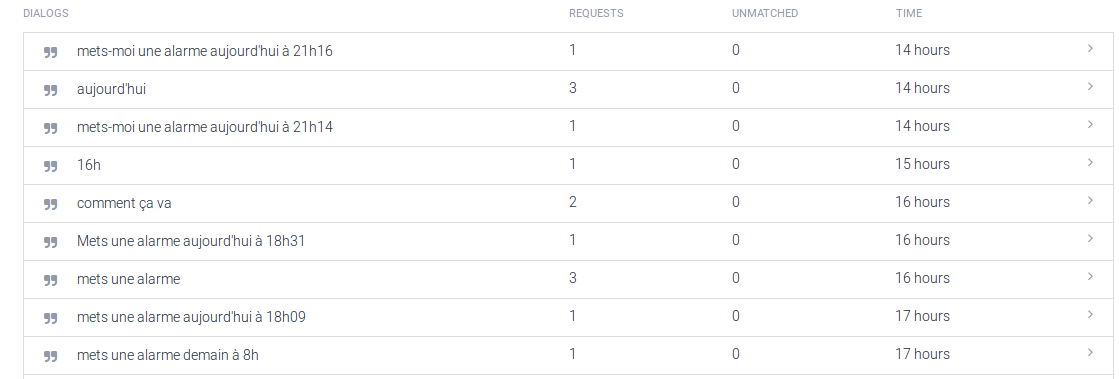
\includegraphics[width=1.2\textwidth]{images/training.png}
        \caption{Onglet entraînement de notre agent}
        \label{training}
\end{figure}


\subsubsection{Serveur REST}

Maintenant que le système de dialogue de notre agent assistant est opérationnel, nous devons mettre en relation l'utilisateur avec ce dernier. DialogFlow propose une API REST très pratique
qui nous permet de converser avec notre agent \emph{via} des simples requêtes HTTP. Chaque conversation différente avec l'agent est identifiée grâce à son identifiant de session,
qui lui est attribué lors de sa création. Cela permet de gérer très facilement les \emph{contextes}.\\

Notre serveur servira donc de \og sur-couche \fg{} qui uniformisera l'échange entre le client et DialogFlow. Écrit en \textbf{Node.js} avec son module \textbf{Express.js}, nous avons fait en sorte qu'il mette à disposition du client deux \emph{endpoints} :\\
\begin{itemize}
    \item \textbf{/dialog/create} : ce \emph{endpoint} sert à créer un dialogue
    \begin{itemize}
        \item méthode : POST
        \item body JSON
        \begin{lstlisting}[language=Javascript]
{
    "text": "la 1ere replique de l'utilisateur"
}
        \end{lstlisting}
    \end{itemize}
    \item \textbf{/dialog/{id}/add} : ce \emph{endpoint} sert à ajouter à une conversation \og id \fg{} une entrée.
    \begin{itemize}
        \item méthode : PUT
        \item body JSON
        \begin{lstlisting}[language=Javascript]
{
    "text": "la 1ere replique de l'utilisateur"
}
        \end{lstlisting}
    \end{itemize}
\end{itemize}


Si notre agent assistant détecte que l'intention est complète (i.e. les \emph{tags} sont tous extraits), alors notre serveur retourne la réponse HTTP suivante :\\

\begin{lstlisting}[language=Javascript]
{
    "sessionId": "sessionId",
    "text": "la reponse de l'agent",
    "confirm": true,
    "type": "action",
    "action": {
        "type": "alarm",
        "datetime": "YYYY-MM-dd HH:mm:ss"
    },
    "error": true|false,
}
\end{lstlisting}

Sinon, il retourne cette réponse : \\

\begin{lstlisting}[language=Javascript]
{
    "sessionId": "sessionId",
    "type": "text",
    "text": "la reponse de l'agent",
    "confirm": false,
    "error": true|false,
}
\end{lstlisting}

De cette façon, l'application client peut connaître très facilement l'état d'un dialogue et donc agir en conséquence.\\

\subsubsection{Intégration}

Afin de faciliter le développement de notre application mobile, nous avons demandé à l'INSA de nous prêter un serveur pour que nous puissions y intégrer notre
application REST. Une fois l'API REST complétement développée et disponible \emph{via} l'adresse du serveur prêté (\url{insa-17-ihme@insa-rouen.fr}), nous avons pu développer
notre application mobile de façon indépendante et sans néccessiter d'avoir une instance de notre serveur REST qui tourne en local.

\subsection{Application mobile}

Comme indiqué plus haut, nous avons choisis de développer notre application mobile en \textbf{react-native}. Facile à prendre en main, \textbf{react-native} possède
plein d'outils déjà tout fait pour gérer les entrées et sorties d'un système de dialogue et pour communiquer efficacement avec une API REST.\\

L'application propose donc simplement une interface permettant de dialoguer avec notre agent assistant \emph{via} une entrée textuelle ou \emph{via} une entrée vocale (microphone du mobile).

Elle possède également une sortie audio pour que l'agent puisse communiquer via la voix avec l'utilisateur, en plus du système de \emph{Chat}.

~\\\indent
L'agent est simplement représenté par une petite icône situé à coté de chacune de ses réponses.

\section{Résultats}

Nous avons répondu à l'ensemble des problématiques et objectifs du projet, et l'ensemble de notre système est fonctionnel et opérationnel. Voici comment utiliser notre prototype : \\

Dans la suite, voici des icônes en figures \ref{hand} et \ref{voice} qui donneront des informations sur les différentes figures de l'application.

\begin{figure}[H]
  \centering
  
\includegraphics[width=2cm]{images/hand.png}
  \caption{Cette icône indique soit un endroit où cliquer à l'écran du \emph{SmartPhone}, soit attire l'attention sur un détail en particulier.}
  \label{hand}
\end{figure}

\begin{figure}[H]
  \centering
  
\includegraphics[width=2cm]{images/voice.png}
  \caption{Cette icône indique l'utilisation du microphone du \emph{SmartPhone}.}
  \label{voice}
\end{figure}

Voici l'écran principal de l'application lors de son ouverture :\\

\begin{figure}[H]
  \centering
  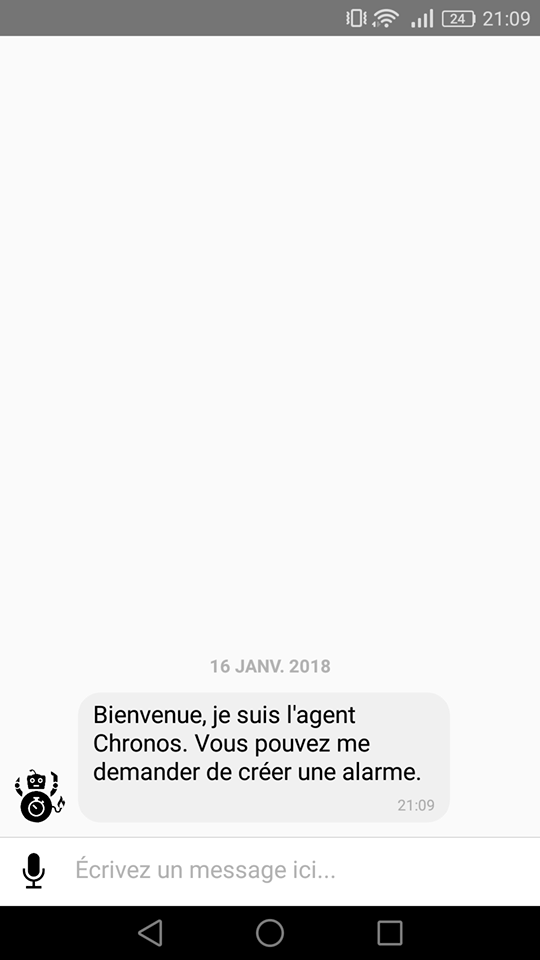
\includegraphics[width=6cm]{images/B1.png}
  \caption{Ecran principal}
  \label{B1}
\end{figure}

Vous pouvez communiquer avec l'agent \emph{via} le microphone en appuyant une fois sur l'icône de micro
ou directement en entrant le texte dans le champ texte se situant à coté de l'icône de micro.

~\\\indent Vous n'êtes pas obligé de donner à l'agent l'ensemble des données
dont il a besoin pour configurer votre alarme \--- en effet vous pouvez très bien y aller étape par étape comme nous allons le voir.

~\\\indent Vous pouvez commencer par cliquer
une fois sur l'icône micro et dire que vous désirez mettre une alarme (figures \ref{B} et \ref{C}).

\begin{figure}[H]
  \centering
  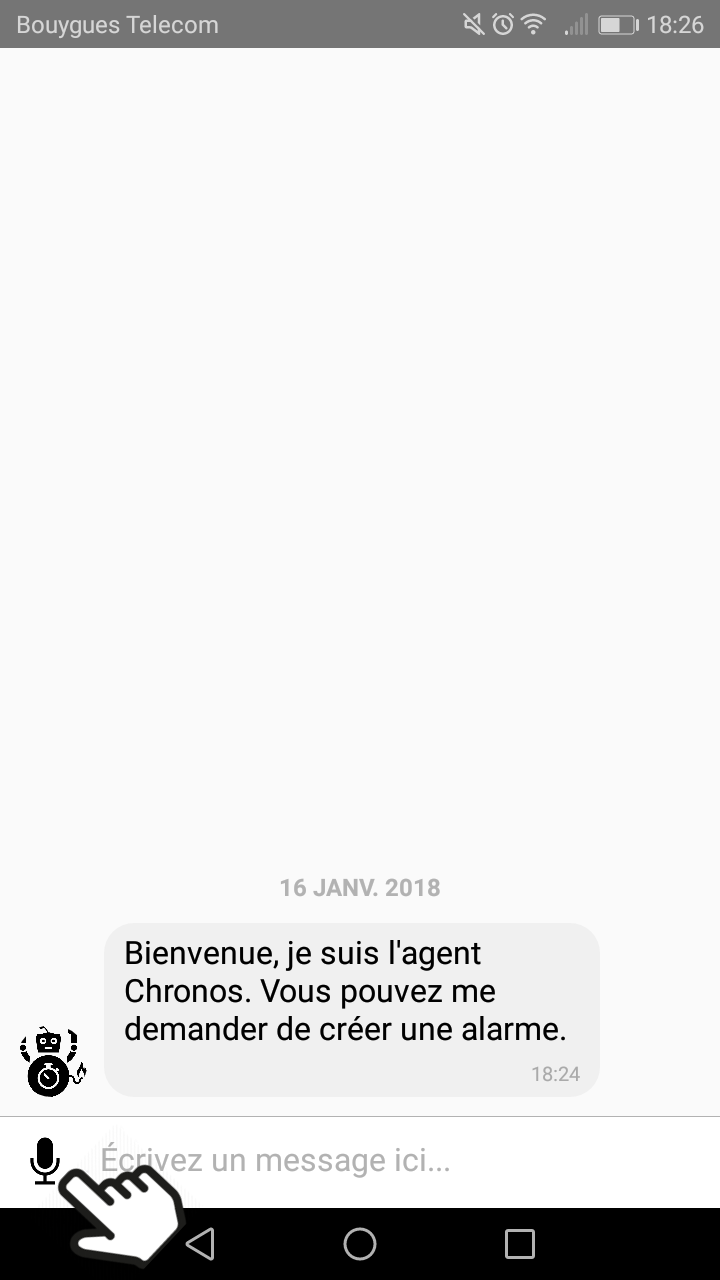
\includegraphics[width=6cm]{images/B.png}
  \caption{Cliquer sur l'icône micro}
  \label{B}
\end{figure}

\begin{figure}[H]
  \centering
  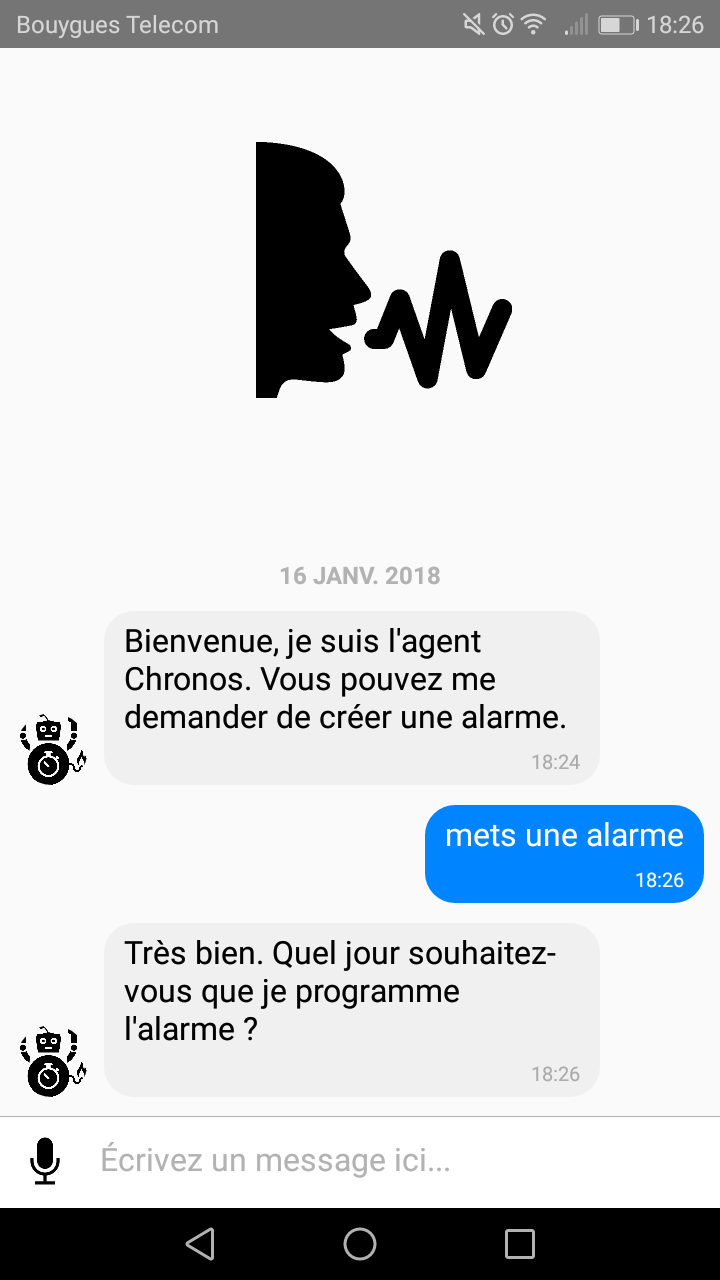
\includegraphics[width=6cm]{images/C.png}
  \caption{Demander la programmation d'une alarme avec la voix}
  \label{C}
\end{figure}

L'application détectera automatiquement que vous avez cessé de parler, vous n'avez donc pas besoin de ré-appuyer sur l'icône micro pour signaler la fin de votre phrase.

~\\\indent Ensuite, vous pouvez indiquer la date à laquelle déclencher l'alarme en cliquant de nouveau sur l'icône micro (figure \ref{D}).

\begin{figure}[H]
  \centering
  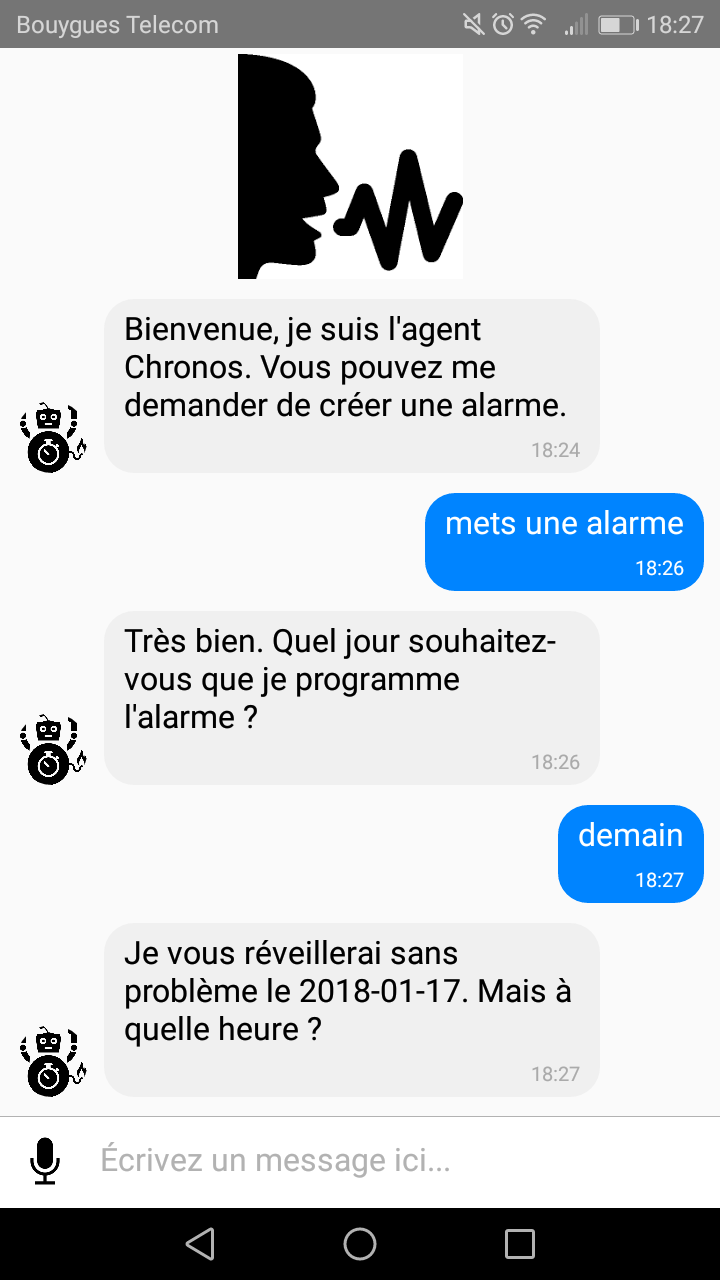
\includegraphics[width=6cm]{images/D.png}
  \caption{Indiquer la date avec la voix}
  \label{D}
\end{figure}

Puis pour finir en lui indiquant l'heure à laquelle déclencher l'alarme.

~\\\indent S'il a bien reconnu votre intention, l'agent vous demandera ensuite une confirmation comme l'illustre la figure \ref{E}.

\begin{figure}[H]
  \centering
  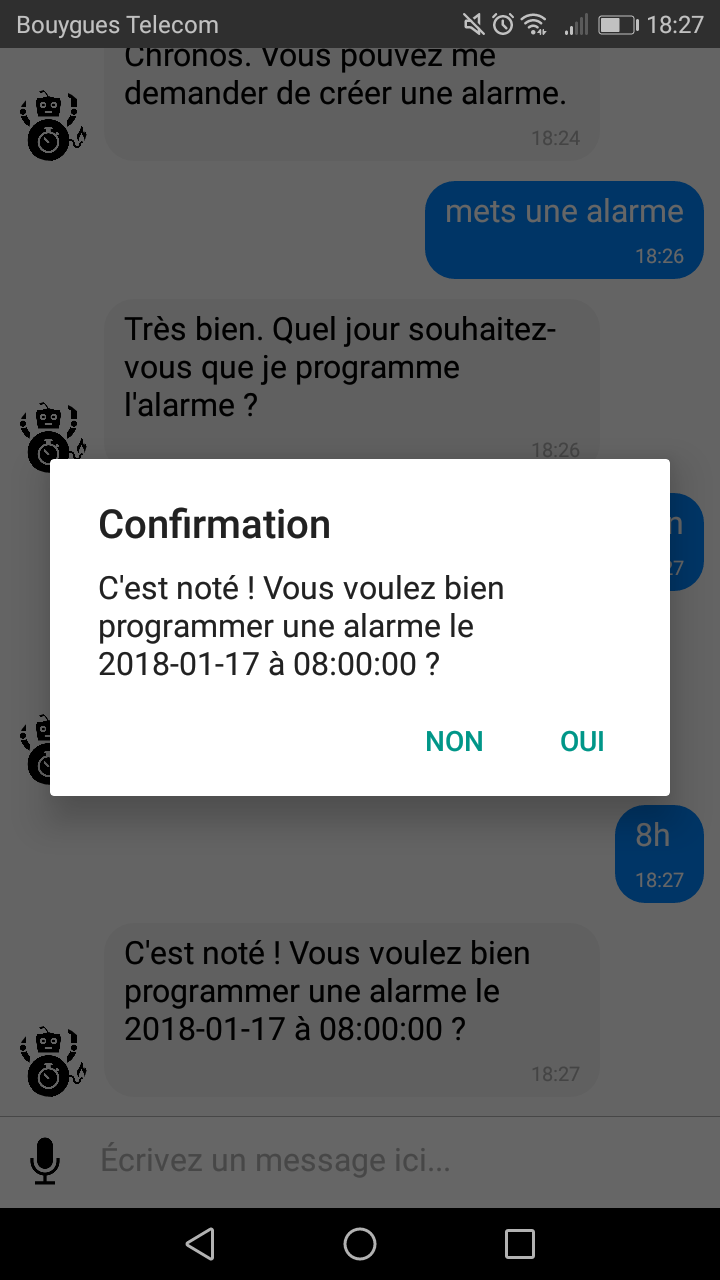
\includegraphics[width=6cm]{images/E.png}
  \caption{Indiquer l'heure et écran de confirmation}
  \label{E}
\end{figure}


Vous auriez très bien pu converser avec l'agent via l'entrée textuelle, comme le représente la figure \ref{F}.

\begin{figure}[H]
  \centering
  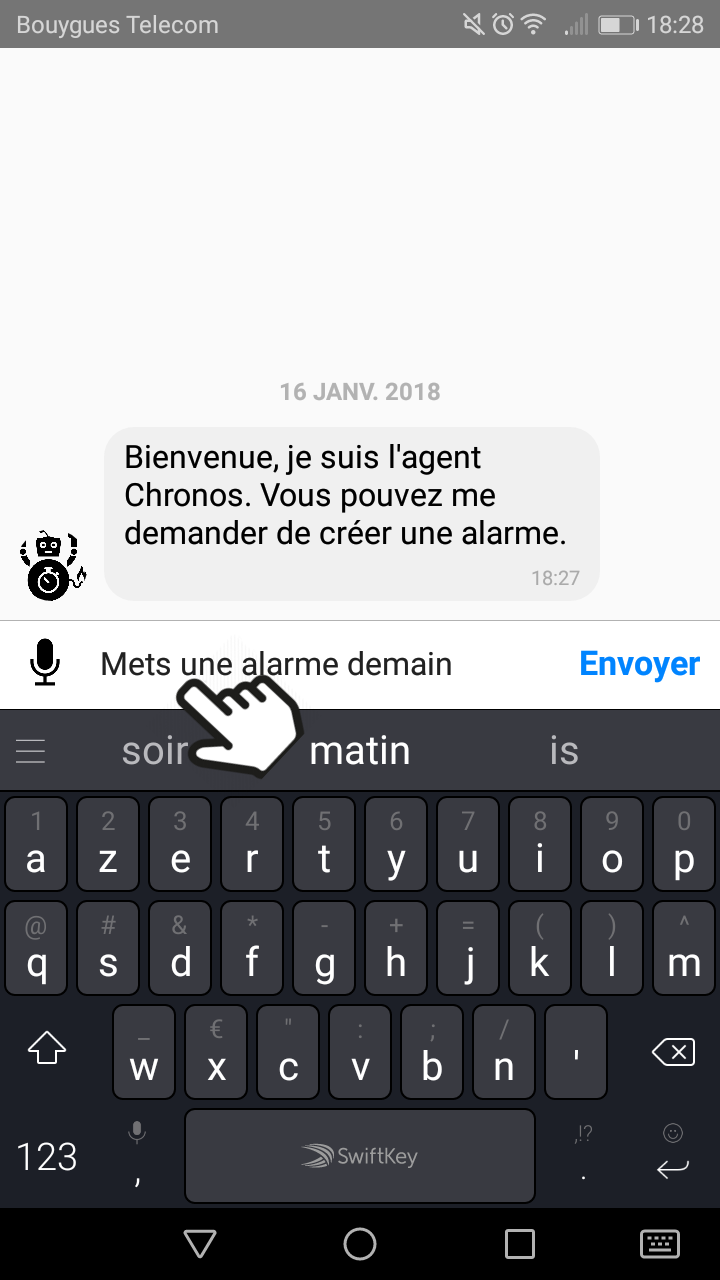
\includegraphics[width=6cm]{images/F.png}
  \caption{Demande de programmation d'une alarme \emph{via} texte}
  \label{F}
\end{figure}

Si vous avez confirmé la programmation de l'alarme, l'agent enregistrera votre demande. Une minute avant le déclenchement de l'alarme demandée, il vous indiquera la météo associée à votre géolocalisation.

~\\\indent
Comme le montre la figure suivante, vous pouvez également programmer l'alarme en une seule phrase si celle-ci est complète (figure \ref{G}).

\begin{figure}[H]
  \centering
  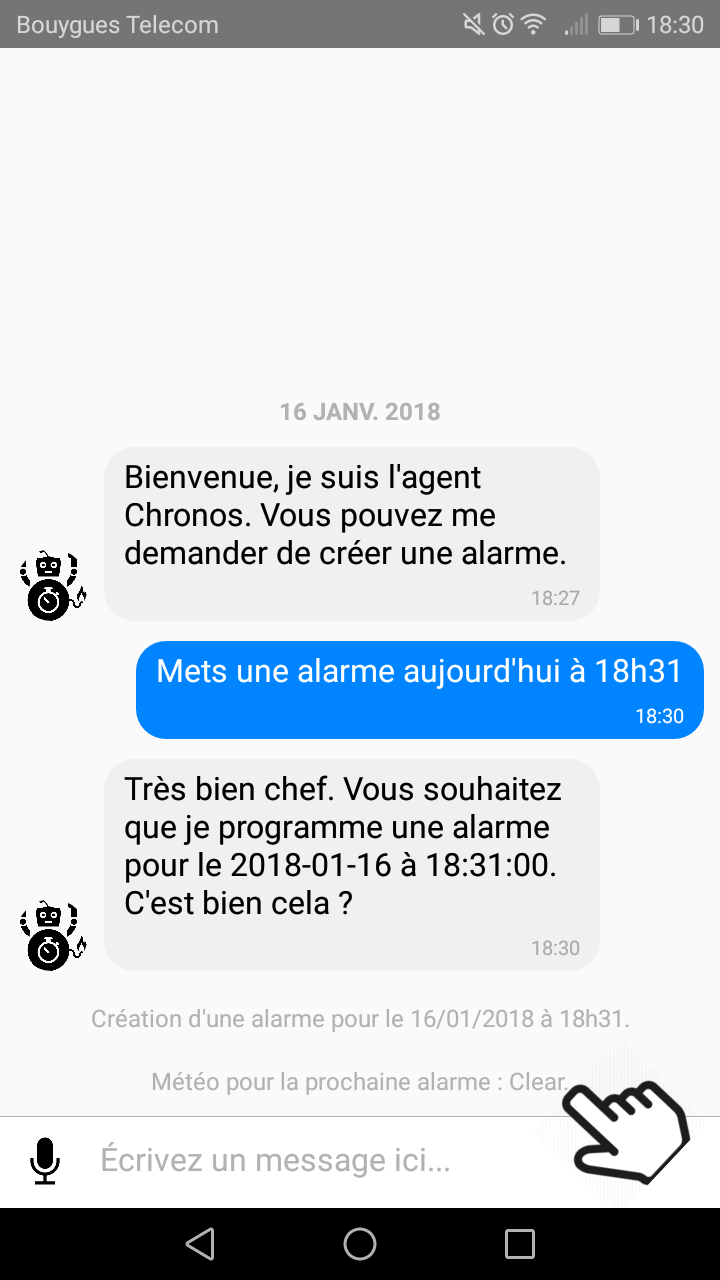
\includegraphics[width=6cm]{images/G.png}
  \caption{Météo associée à l'alarme}
  \label{G}
\end{figure}

Lorsque qu'une alarme se déclenchera, vous recevrez une notification accompagnée de la musique associée à la météo liée à votre localisation (figure \ref{H}).

\begin{figure}[H]
  \centering
  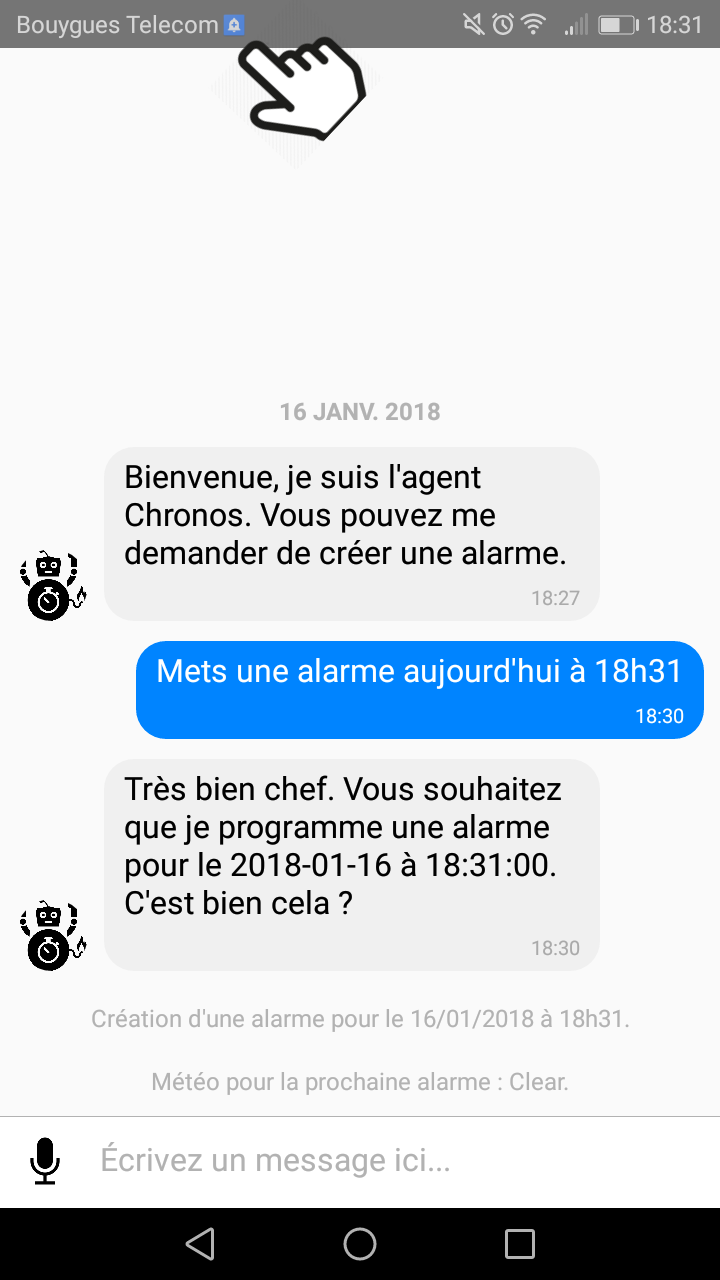
\includegraphics[width=6cm]{images/H.png}
  \caption{Déclenchement d'une alarme : notification}
  \label{H}
\end{figure}

~\\\indent
\textbf{Petit bonus :} l'agent reconnaîtra quelques phrases supplémentaires non liées aux fonctionnalités prévues initialement pour l'application (figure \ref{J}), à vous de les découvrir \textsf{;)}.

\begin{figure}[H]
  \centering
  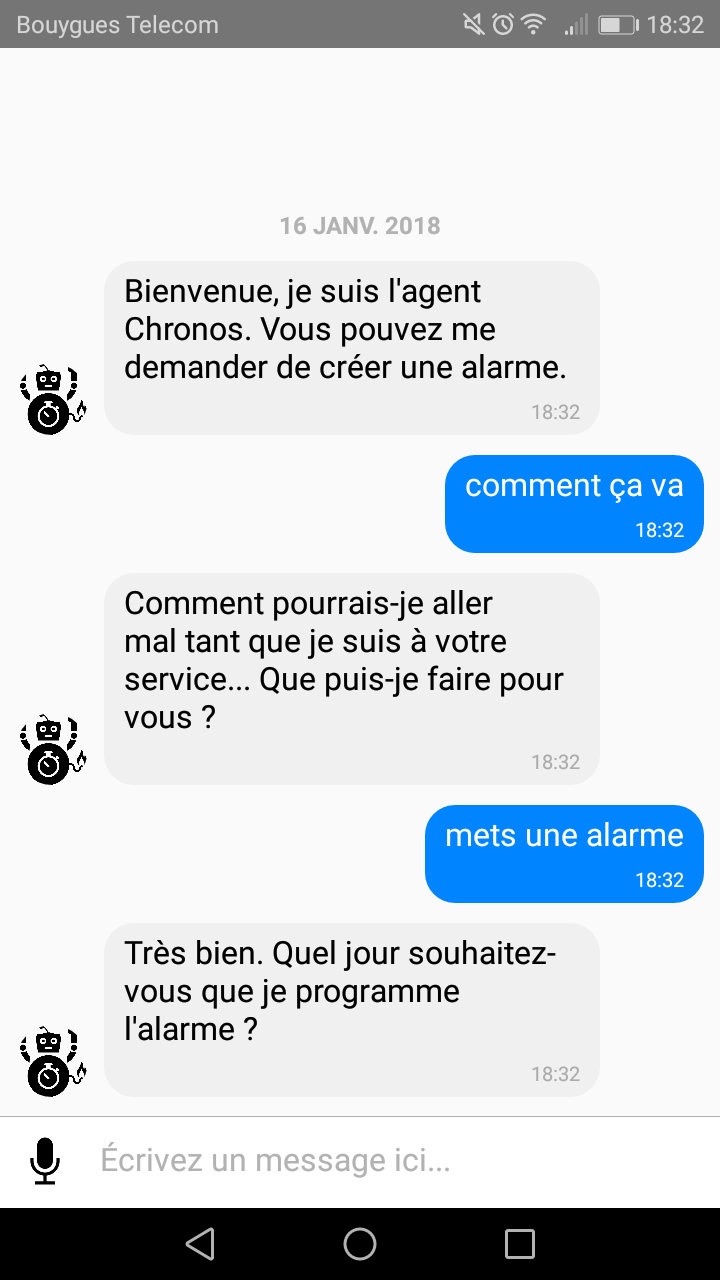
\includegraphics[width=6cm]{images/J.png}
  \caption{Petite conversation bonus}
  \label{J}
\end{figure}

Une vidéo de démonstration est également disponible avec ce rapport et est située dans le dossier \emph{demo} à la racine du projet.\\
